\chapter{Application for design-space~exploration}
\label{chap:apply}

To achieve our goal of supporting design-space exploration with stochastic metrics, a formalism for the convenient modular construction of stochastic models was presented in the previous chapters along with a technique for transforming engineering (architectural) models into stochastic models. Now the application of these tools in design-space exploration (\textabbr{DSE}) toolchains is discussed.

Users may configure the model transformation framework proposed in \cref{chap:transform} by providing a transformation description, which determines the source \textabbr{DSL} and the \textabbr{RGSPN} fragments instantiated by transformation according to source model. Integrating the transformation engine into a \textabbr{DSE} pipeline enables running any such transformation description to provide analysis models.

Queries associated with the analysis models are represented as variables in the \textAbbr{RGSPN}s derived by our transformation. The answers to the queries, which can calculated by external stochastic analysis tools, guide the \textabbr{DSE} process as constraints to satisfy and goal functions to optimize. To carry out the computation the design space explorer must interface with the analysis tools. Serialization in \textabbr{ISO}/\textabbr{IEC}~15909-2:\citeyear{ISO1590922011} \textabbr{PNML} format was provided for interoperability with externals tools. However, the toochain integrator must provide means to run the external solver, to serialize stochastic queries in its input format and to read the analysis results.

As the literature pertaining the optimization of stochastic models was already reviewed in \vref{sec:intro:relwork}, in this chapter we start by describing the tasks related to the integration of our analysis model transformation framework with a \textabbr{DSE} toolchain. In addition, we describe the implementation of the framework along with the interfaces provided to users and our empirical evaluation of its scalability.

\section{Integration with design-space exploration toolchains}

\citet{Kang10effective} have identified cornerstones of an effective \textabbr{DSE} framework as
\begin{inparaenum}
\item a suitable \emph{representation} of the design space,
\item \emph{analysis} capabilities to check discovered potential candidates against design constraints and
\item an \emph{exploration method} for navigating interesting solutions.
\end{inparaenum}
The approaches and representations used for \textabbr{DSE} in the context of model-driven engineering were further classified by \citet{Vanherpen14patterns}. They have identified the following \emph{\textabbr{DSE} patterns} of exploration methods:
\begin{itemize*}
\item The \emph{Model Generation Pattern} synthesizes design candidates that satisfy a set of constraints, which are imposed based on the metamodel and in addition by the designer. During the exploration, design candidates are represented as solutions of a constraint satisfaction problem. Tools based on this pattern include \textabbr{FORMULA}~\citep{Kang10effective} and Alloy Analyzer~\citep{Jackson11abstractions}.
\item The \emph{Model Adaptation Pattern} constructs an exploration representation, such as a string of genes in genetic algorithms~\citepeg{Ferrandi08multiobjective} from an initial model provided by the designer. Based on the guidance of a goal function further design candidates are devised in this intermediate form using (meta-)heuristic search.
\item The \emph{Model Transformation Pattern} directly represents the design candidates as an instance model. Model transformation rules that yield alternative models are scheduled using (meta-)heuristics to optimize a goal function. An example of this approach is \textabbr{VIATRA-DSE}~\citep{Hegedus13guided,Abdeen14multiobjective}.
\item The \emph{Exploration Chaining Pattern} adds multiple abstraction layers to \textabbr{DSE} to prune the space of alternative solutions. At each abstraction layer, an exploration pattern is used to prune non-feasible solutions while selecting feasible solutions to be refined in the next layer. Domain knowledge is used to define abstraction layers. Costly evaluation of design candidates is usually deferred to the lower layers.
\end{itemize*}

\citet{Vanherpen14patterns} also classified the representations employed by \textabbr{DSE} patterns:
\begin{enumerate*}
\item The starting point for exploration is expressed in a \emph{model} formalism.
\item Constraints to be satisfied by the design alternatives and objective function to be optimized are captured by \emph{constraint} and \emph{goal} formalisms.
\item Design candidates are stored in an \emph{exploration formalism} during the exploration. In the \emph{Model Transformation Pattern}, this coincides with the \emph{model} formalism.
\item The exploration formalism may be transformed into an \emph{analysis} formalism to check feasibility with respect to the constraints.
\item A second transformation may target a \emph{performance} formalism to check optimality with respect to the goal functions.
\item Execution traces yielding the design alternatives are stored in a \emph{trace} formalism.
\item Finally, the solution is output in a \emph{solution} formalism, which may coincide with either the model or the trace formalism.
\end{enumerate*}

The \textabbr{RGSPN} formalism proposed in \cref{chap:rgspn} may serve as both an \emph{analysis} formalism when constraints are formulated in terms of stochastic analysis queries and as a \emph{performance} formalism when the optimized goal function is a stochastic metric. Hence in \textabbr{DSE} the transformation proposed in \cref{chap:transform} should be employed as a means of transforming models in the \emph{exploration} formalism to the \emph{analysis} formalism. In more elaborate transformation chains, where a separate analysis formalism is employed and \textAbbr{RGSPN}s are only used as \emph{performance} formalism, the \emph{analysis} formalism may serve as a source instead. The traceability links produced by the transformation ensure that the results of the analysis can be interpreted as information about the satisfaction of constraints and the values of goal functions defined over the engineering formalisms.

The proposed approach based on incremental model transformation is especially suited for the \emph{Model Transformation} \textabbr{DSE} pattern, where the change-driver mapping to \textAbbr{RGSPN}s can be performed directly from the \emph{model} formalism. Hence the same mapping is applicable for both stand-alone engineering models and in \textabbr{DSE}, while the change-driver transformation may react to source model changes caused by the exploration rules. The transformation description, which specifies the creation of \textAbbr{RGSPN}s from the \emph{model} formalism, can serve as the \emph{constraint} or \emph{goal} formalism, since it encodes which stochastic queries are constructed and evaluated for the instance models.

For application in the context of \emph{Model Generation} and \emph{Model Adaptation} the transformation description for our analysis transformation engine must be formulated with the \emph{exploration} or an intermediate \emph{analysis} formalism as the source. The resulting transformation will be only suitable for \textabbr{DSE} and not for standalone model mapping. Moreover, in \emph{Model Generation} change-driven incrementality may have diminished utility, because constraint solvers often generate solution in the \emph{exploration} formalism from scratch instead of applying change operations. Adaptation of constraint solvers to the incremental setting is challenging due to scalability issues~\citep{Semerath16generation}, especially in the case of graph generation with complex structural constraints~\citep{Semerath16backward}.

\begin{remark}
  A recent approach in \emph{Model Generation} combines partial interpretations from mathematical logic and techniques from Boolean satisfiability (\textabbr{SAT}) solvers to formulate the problem in terms of \emph{Model Adaptation}~\citep{Varro17generation}. The \emph{exploration} formalism in this approach is a partial interpretation of the original \emph{model} formalism. It is possible to evaluate model queries on the partial interpretation by constraint rewriting of queries over the original \emph{model} formalism~\citep{Semerath17rewriting}. Therefore our transformation engine could be adapted to construct \textAbbr{RGSPN}s from the partially interpreted \emph{exploration} formalism based on a transformation description developed for the original \emph{model} language by rewriting (\enquote{lifting}) the involved model queries, which would enable incremental execution in all three major \textabbr{DSE} paradigms.
\end{remark}

\begin{remark}
  Retaining parameter symbols in \textAbbr{RGSPN}s for use with external solvers provides an opportunity for \emph{Exploration Chaining}. The elements of the \textabbr{CTMC} parameter vector \(\vec{\uptheta} \in \mathbb{R}^{\lvert \Par \rvert}\) correspond to primitive attributes of engineering model elements after transformation. Hence the vector is a concise \emph{exploration} representation of a design alternative once its structure is fixed and only attributes need to be filled in. As a nested exploration method, algorithms based on sensitivity analysis and numerical optimization~\citep{Molnar17optimization} or parametric abstractions~\citep{Quatmann16mdp} may be employed so that the higher-level exploration method can be reserved to propose candidate structures for the design. 
\end{remark}

\subsection{Model transformation based design-space explorers}

Incremental transformation to \textabbr{RGSPN} analysis models was considered above in the contexts of various \textabbr{DSE} patterns. We now describe the operation of our transformation engine with the \emph{Model Transformation Pattern}, which is perhaps the most amenable to change-driven synchronization of analysis models.

\begin{figure}
  \centering
  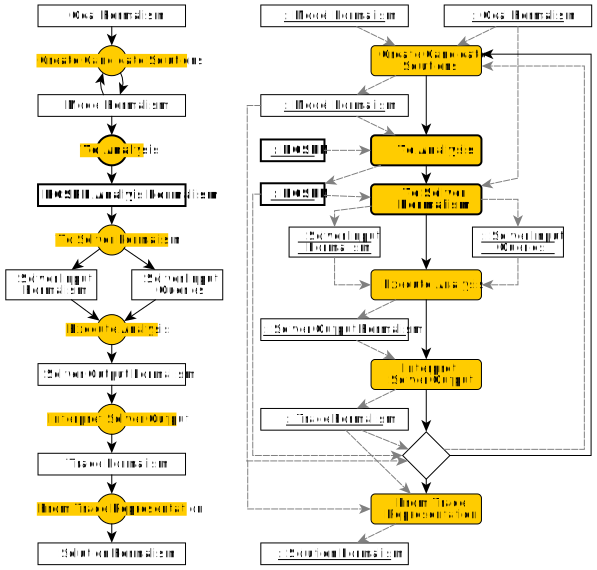
\includegraphics[scale=0.9]{figures/dse_ftg_pm}
  \caption{\textabbr{FTG+PM} of the \emph{Model Transformation} \textabbr{DSE} pattern with \textabbr{RGSPN}-based analysis. The components in \textbf{bold} were implemented in our work, while the rest of the components should be supplied by the \textabbr{DSE} framework and stochastic analysis tool.}
  \label{fig:apply:ftg-pm}
\end{figure}

The Formalism Transformation Graph and Process Model (\textabbr{FTG+PM}) notation was proposed by \citet{Lucio12ftgpm} as a guide to carry out model transformations in multi-paradigm modeling. An  extended version of the \emph{Model Transformation Pattern} \textabbr{FTG+PM} of \citet[Figure~4]{Vanherpen14patterns} is shown in \cref{fig:apply:ftg-pm}, which illustrates model transformation based \textabbr{DSE} with incrementally synchronized \textabbr{RGSPN} analysis models. The Formalism Transformation Graph (\textabbr{FTG}) on the left shows the modeling languages as rectangles and the involved model transformations as circles. Arrows indicate the direction of transformations, such that bidirectional arrows correspond to in-place model modification. The Process Model (\textabbr{PM}) contains the transformation activities, which are displayed as rounded rectangles, their control flow (solid arrows) and data flows (dashed arrows). Languages and transformations provided by our framework are emphasized in bold.

Model transformation based \textabbr{DSE} works directly on the \emph{model} formalism. Heuristics or meta-heuristics provided by the \textabbr{DSE} toolchain in the \emph{Create Candidate Solutions} activity apply model transformations according to some goal functions. In order to support change-driven synchronization of the \textabbr{RGSPN} view for analysis, the transformations should be in-place so that change notifications can be propagated. In the \textabbr{PM}, the in-place model modification is indicated by data flows of pieces of input and output data of the same type.

The \emph{To Analysis} activity derives the \textabbr{RGSPN} analysis model by interpreting the transformation description in the \emph{goal} formalism with our transformation engine, which was described in \cref{chap:transform}. The analysis models are derived incrementally by modifying the \textAbbr{RGSPN}s in place according to changes in the candidate solution. The resulting \textAbbr{RGSPN} contains both the stochastic analysis model and the variable symbols that correspond to the goal functions.

The queries pertaining goal functions and queries can be answered on the analysis model by executing the stochastic analysis in an external tool. The \textabbr{RGSPN} model is transferred to the external tool by serializing it in a standardized interchange format, which is the \emph{Solver Input Formalism}. Moreover, the queries themselves must be serialized in the appropriate \emph{Solver Input Query} formalism. The \emph{To Solver Representation} activity performs this task. We provide an implementation of this activity as part of our framework that targets them \textabbr{ISO}/\textabbr{IEC}~15909-2:\citeyear{ISO1590922011} \textabbr{PNML} format as the \emph{Solver Input Formalsm} while using extensions defined by the PetriDotNet tool~\citep{Voros17pdn} to convey timings of Petri net transitions and stochastic queries.

After the \emph{Execute Analysis} activity, which usually involves calling an external program, the answers to the stochastic queries are obtained in the \emph{Solver Output Formalism}. This representation must be parsed in the \emph{Interpret Solver Output} activity so that the values of the goal functions are available to the \textabbr{DSE} toolchain. The \textabbr{DSE} toolchain incorporates the results of the analysis into the \emph{trace} representation; thus the candidate designs in the solution store can be compared according to their fitness.

The \emph{Model Transformation} \textabbr{DSE} pattern is iterative. The traces, which are enriched with the values of the goal functions, are incorporated by the \emph{Create Candidate Solutions} heuristics to produce new design candidates. The in-place modification of the candidate design and the \textabbr{RGSPN} is signified in the \textabbr{PM} by the data flow going into the decision node at the end of the loop and the data flow back to the start of the loop.

Finally, if required, the optimal solution or a set of solutions can be transformed from the trace representation to the \emph{solution} formalism by the \emph{From Trace Representation} activity.

\subsection{Stochastic analysis tools}

To answer the queries posed as variable symbols in the \textabbr{RGSPN} analysis models external stochastic analysis tools must be invoked. As discussed in the previous section, this requires a modification of the \textabbr{DSE} toolchain to produce input for the external tool, invoke it and parse its output. However, additional support for this workflow must be incorporated into the analysis tool, too.

Firstly, the analysis tool needs to have an interface for unattended execution. Various ways to provide this interface include command-line applications and web services. For example, the PetriDotNet analysis tool contains a separate binary executable for running stochastic analyses in the command line.\footnote{This tool, similarly to the rest of PetriDotNet~1.5b2 is available from \url{https://inf.mit.bme.hu/en/research/tools/petridotnet} upon request. More information can be found in the user manual by \citet{Voros17pdnmanual}.} While initiatives such as the Model Checking Contesti~(\textabbr{MCC})~\citep{Kordon17mcc} and the Petri Nets Repository~\citep{Hillah17repository} strive for common interfaces for Petri net analysis tools, to our best knowledge, no generic interface is widely supported. Hence even though models serialized in the \textabbr{PNML} format are portable between solvers, each of them must be called in a specific way.

Secondly, any parameters required by the analysis in addition to the stochastic model and the queries must be supplied automatically. For stochastic Petri net analysis, these parameters include the ordering of state variable in symbolic analysis methods when the model is converted into a \textabbr{CTMC} and the choice of numeric algorithm to solve the arising systems of linear or differential equations.

\subsubsection{Variable ordering}

Symbolic computations methods such as \emph{saturation}~\citep{Ciardo01saturation,Ciardo12tenyears} are often used in the state-space exploration of Petri nets, which is required for model checking logical properties and the construction of \textAbbr{CTMC}s from stochastic Petri nets~\citep{Miner04mdd}. Symbolic algorithms represent the reachable state space of the formal model as a \emph{decision diagram}, such as a multi-valued decision diagram (\textabbr{MDD})~\citep{Kam98mdd}. The decision diagram is a directed acyclic graph where each node belongs to a given \emph{level}. Each state variable of the model, which may be the marking of single place or a collection of places in Petri nets, is assigned to a different level. The assignment is referred to as the variable \emph{ordering}. Outgoing edges from nodes are labeled with the possible values of the state variable, such that each path in the graph is a reachable state, i.e.~a reachable Petri net marking.

The transitions in the formal model induce a next-state relation over the states in the diagram. The reachable state space can be determined by fixed-point iteration of the next-state relation. By selecting appropriate representation of the next-state relation, even complex models, such as stochastic Petri nets with immediate transition priorities can be handled~\citep{Miner06saturation,Marussy17priorities}. However, the variable ordering has dramatic effects on the run time of the fixed point computation~\citep{Amparore17ordering}. Stochastic analysis is further made difficult due to the decompositions employed in the numerical solution of \textAbbr{CTMC}s often requiring variable assignments that differ from those suitable for symbolic analysis~\citep{Marussy16decompositions}.

As the structure of the derived Petri net model may constantly change during exploration, the variable ordering cannot be provided to the solver manually. Either the solver itself or some other component of the \textabbr{DSE} pipeline must generate an acceptable variable ordering. Based on the abstraction level at which the generation is done, we suggest three possible solutions as follows:
\begin{itemize*}
\item The stochastic analysis tool itself may generate a variable order by some heuristic, such as those surveyed by \citet{Amparore17ordering}.
\item The \textabbr{RGSPN} transformation engine may communicate the groupings of places induced by the instantiation of Petri net modules to the analysis tool. The nested-unit Petri net (\textabbr{NUPN}) format was proposed by \citet{Garavel15nupn} to encode such grouping and was employed in the 2017 edition of the \textabbr{MCC} to aid variable ordering heuristics of the participating tools~\citep{Kordon17mcc}.\footnote{The specification for embedding \textabbr{NUPN} data in \textabbr{PNML} files is available at \url{https://mcc.lip6.fr/nupn.php}.}
\item It would be also possible to extend the transformation specifications such that our transformation engine could generate variable orderings along with \textAbbr{RGSPN}s.
\end{itemize*}

\subsubsection{Numerical algorithm selection}

Another setting which may dramatically impact the solution time and accuracy of stochastic models is the choice of the numerical algorithms.

In stead-state and mean time to state partition analysis, solving the \textabbr{CTMC} reduces to a system of linear equations, where the number of variables and equations equal to the size of the reachable state space of the model. The matrix of this system of linear equations is the \emph{infinitesimal generator matrix} of the \textabbr{CTMC}, which is sparse and often amenable to decomposed storage~\citep{Buchholz99hierarchical}.

Due to the size of the systems direct solution methods are infeasible and iterative numerical methods are employed instead. However, the choice the iterative linear equations solver method and its parameters determines the run time and convergence of the solution; moreover, no numerical method was found to be suitable for all classes of models~\citep{Buchholz99structured,Marussy16configurable,Buccholz17compact}.

In transient analysis, transitions with orders of magnitude timing difference cause \emph{stiffness} the system of differential equations associated with the \textabbr{CTMC}. Stiff Markov chains may be handled by numerical differential equation solver algorithms especially tailored to such situations~\citep{Reibman89transient} or by adaptive variants of the \emph{uniformization} algorithm~\citep{Moorsel97uniformization,Dijk17uniformization}.

To our best knowledge, no method was proposed in the literature to automatically select a suitable numeric algorithm for stochastic analyses. An analysis tool may offer a default selection; however, for ill-conditioned problems, the user should override it before starting design-space exploration. Alternatively, a portfolio of algorithms may be specified that are tried sequentially or in parallel until one of them converges successfully.

\begin{remark}
  Deeper, change-driven integration between external analysis tools and model transformation toolchains has been suggested recently by \citet{Molnar16componentwise} and \citet[Section~2.8]{Meyers16thesis} inspired by incremental approaches in the evaluation of expensive model queries~\citep{Ujhelyi15incquery}. Such integration might allow solvers to receive model changes and compute the analysis result incrementally by reusing parts of the previous solution.
  
  Since our \textabbr{RGSPN} transformation is engine is fully change-driven it is able to translate engineering model changes to analysis model changes, which could be sent directly to the solver. Moreover, in the numeric analysis of \textAbbr{CTMC}s it is sometimes possible to reuse the previous solution vector as an initial approximation. However, no existing analysis tool is in our knowledge that is able to take advantage of model change information; therefore extending change-driven execution throughout the analysis remains in the scope of future work.
\end{remark}

\section{Software implementation}

A software tool for the development of transformation specifications and their execution was implemented as a plug-in for the Eclipse Oxygen.1 Integrated Development Environment\footnoteurl{http://www.eclipse.org/downloads/packages/release/Oxygen/1}~(\textabbr{IDE}). The plug-in is based on open source technologies from the Eclipse Modeling Project: the \emph{Eclipse Modeling Foundation}~(\textabbr{EMF})~\citep{Steinberg09emf}, the \emph{XText}\footnoteurl{https://www.eclipse.org/Xtext/} framework for language engineering and \emph{\textabbr{VIATRA}} scalable reactive model queries and transformations.

The software consists of two major components. Both \textabbr{RGSPN} modules and model transformations from arbitrary \textabbr{EMF}-based \textAbbr{DSL}s to \textAbbr{RGSPN}s can be developed in the transformation specification environment. The transformation can be executed either inside the \textabbr{IDE} for testing or inside a \textabbr{DSE} program after Java code generation. Together with a runtime library implementing the transformation engine, the generated Java code provides incremental transformation to stochastic Petri nets from \textAbbr{DSL}s defined with \emph{Ecore} metamodels, the metamodeling core of \textabbr{EMF}.

\subsection{Specification environment}

\begin{figure}
  \centering
  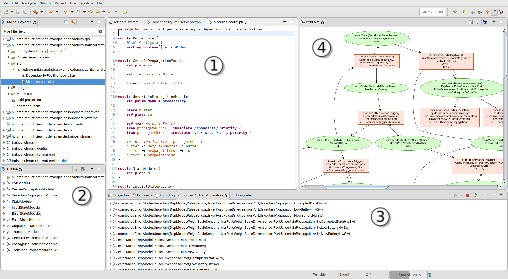
\includegraphics[width={\dimexpr\textwidth-2\fboxrule},frame]{figures/annotated_screenshot}
  \caption{Sreenshot of the transformation specification environment. The showcased features include \circled{1}~the transformation description editor with syntax highlighting, \circled{2}~the outline view for transformations, \circled{3}~the \emph{Ecore2Pn Transformation} execution and traceability viewer and \circled{4}~the \textabbr{RGSPN} graph \emph{Petri Net} visualizer.}
  \label{fig:apply:screenshot}
\end{figure}

A specification development environment named \emph{Ecore2Pn} (Ecore to Petri net transformation) was implemented for \textabbr{RGSPN}-based transformation development.\footnote{The specification development environment was implemented by the author during his summer internship at \emph{ThyssenKrupp Presta Hungary Kft.}} A screenshot of the tool is shown in \vref{fig:apply:screenshot}.

The plug-in suite contains concrete textual syntaxes for \textabbr{RGSPN} modules and transformation descriptions based on the Xtext language engineering framework. Integrated devlopment environment (\textabbr{IDE}) features, such as semantics-aware syntax highlighting, content assist for code completion, jump-to-definition and outline view are available. The definition of model queries as preconditions for the \textabbr{RGSPN} transformation rules is possible with the \textabbr{VIATRA} Query \textabbr{EMF} query definition editor~\citep{Ujhelyi15incquery}.

Similarly to the \textabbr{VIATRA} query editor, integration is offered with the modeling services of the Eclipse \textabbr{IDE} to try out and debug transformation descriptions. The transformation may be executed live on models loaded as \textabbr{XMI}~\citep{OMG15xmi} files or with graphical concrete syntax as Sirius\footnoteurl{http://www.eclipse.org/sirius/} diagrams. Modification of the model triggers change-based synchronization of the \textabbr{RGSPN}. A listing of instantiated \textabbr{RGSPN} modules symbols along with traceability links is displayed in the \emph{Ecore2Pn Transformation} view. Moreover, a graphical view of the \textabbr{RGSPN} is available in the \emph{Petri Net} view.

\subsubsection{Model export}

In addition to transformation development and execution, \emph{Ecore2Pn} offers export facilities for model interchange. These features are part of the transformation engine runtime; therefore they are also available for developers who wish to integrate \textAbbr{RGSPN}s into \textabbr{DSE} toolchains. \emph{Ecore2Pn} merely provides a convenient user interface for exporting single models.

Serialization in \textabbr{ISO}/\textabbr{IEC}~15909-2:\citeyear{ISO1590922011} \textabbr{PNML} format allows model interchange with external analysis tools. The exporter also supports the \emph{state reward configuration} and \emph{fault configuration} facilities of PetriDotNet~\citep[Section~4.2]{Voros17pdnmanual} for Markovian steady-state, transient and mean time to state partition analysis. Symbols marked with the \texttt{@Reward\-Conf{}iguration} and \texttt{@Fault\-Conf{}iguration} annotations in the \textabbr{RGSPN} textual editor get translated into reward and fault configurations, respectively, and are available for analysis once the exported \textabbr{PNML} is opened with PetriDotNet.

An additional export facility is available targeting the \texttt{dot} format compatible with the \emph{Graphviz}\footnoteurl{https://www.graphviz.org/} graph visualization software. The \texttt{dot} utility provides automatic layouting and drawing for directed graphs, which allows visual inspection of \textabbr{RGSPN} models. This exporter is also employed along with a Java port\footnoteurl{https://github.com/nidi3/graphviz-java} of Graphviz by the \emph{Petri Net} view of the specification environment to display the results of the currently running \textabbr{RGSPN} transformation.

\subsubsection{Code generation}

Code generation is used throughout the specification development environment to ensure that the transformation specification can be ran in a wide variety of environments, such as within and Eclipse plugin-in or as a standalone Java application.

The \textabbr{RGSPN} modules and the transformation description defined by the user are turned into Java code for compilation. In this way the transformation description can be passed to the execution engine by just instantiating a class, just like how \textabbr{VIATRA} Query generates pattern-specific matcher code from graph patterns for type-safe consumption~\citep[Section~2.3]{Ujhelyi15incquery}. Moreover, as model queries, \textabbr{RGSPN} modules and transformations become Java classes, their dependencies can be managed by the Java \textabbr{CLASSPATH} mechanism. For example, and \textabbr{RGSPN} module can be seamlessly upgraded by replacing its containing archive on the \textabbr{CLASSPATH} without breaking compatibility with transformation definitions in other archives that refer to the module.

Additional helper code is generated for derived features defined in transformations. The helper enables simulates derived features in code written in the \emph{Xtend}\footnoteurl{https://www.eclipse.org/xtend/} programming language. The \emph{extension methods} feature allows traversal of the traceability relations created by the \textabbr{RGSPN} transformation engine to obtain derived feature symbols as if they were true properties of the domain model elements.

\subsection{Transformation execution}

The transformation execution engine is a Java library than can be used either as an Eclipse plug-in or in standalone applications. The transformation engine can be instantiated with an existing \textabbr{VIATRA} Incremental Query engine over an \textit{\textabbr{EMF} scope} which contains the intended source model. The other argument required for the transformation is the generated transformation specification object, which refers to the \textabbr{VIATRA} model queries and \textabbr{RGSPN} modules involved in the transformation. Once instantiated, the engine executes in an incremental fashion and reacts to changes in the source model.

It is possible to only execute the view transformation, which yields an abstract \textabbr{RGSPN} with collections and references, or both the view and the concretizer transformation, which also yields a concrete \textabbr{RGSPN} that can be exported to external analysis tools. The engine can be customized by overriding \emph{Google Guice}\footnoteurl{https://github.com/google/guice} dependency injections.

Traceability relations can be traversed either by explicitly reading them, or by the derived features helper classes generated for Xtend programming. In addition, extra \emph{annotations} specified in the \textabbr{RGSPN} modules and the transformation description are also propagate through the transformation chain, which may influence the behavior of \textabbr{RGSPN} exporters.

\section{Evaluation of incremental transformations}

We carried out preliminary scalability evaluation of our transformation runtime in order to study the overhead the imposed on transformation imposes on design-space exploration. Both \emph{batch execution}---where the transformation engine is initially instantiated and the intermediate and target \textabbr{RGSPN} models are materialized according to the engineering models---and \emph{incremental execution}---where each source model change is immediately translated into intermediate and target model changes---were studied. More specifically, we carried out the evaluation in the \emph{dining philosophers} domain to address the following three research questions:
\paragraph{\textabbr{RQ1}} How does the initial batch transformation from the engineering \textabbr{DSL} to the formal stochastic model (\textabbr{GSPN}) scale with respect to size of the input model?
\paragraph{\textabbr{RQ2}} How does the incremental transformation scale with respect to the size and the change operations of the input model?
\paragraph{\textabbr{RQ3}} What is the overhead associated with the serialization of models to the \textabbr{ISO}/\textabbr{IEC} \textabbr{PNML} interchange format?

\newpara Answering these questions may help identifying strengths and weaknesses of the proposed approach to the stochastic evaluation of engineering models. Moreover, the answers to \textbf{\textabbr{RQ1}} and  \textbf{\textabbr{RQ2}} aid in determining whether incremental or batch model transformation should be used according to the usual size of source changes. This choice arises when there is no need to construct the target model change as a sequence of operations for each source change; therefore incremental execution is not necessitated and the system integrator can chose between either execution schemes. Lastly, the answer to \textbf{\textabbr{RQ3}} tells whether the overhead of serialization into a portable format is acceptable or more direct integration and communication with the external solver is needed.

\subsection{Measurement setup}

\begin{table}
  \caption{Source model, abstract net and concrete net sizes for the philosophers models.}
  \label{tbl:apply:model-size}
  \sisetup{table-number-alignment=center}
  \centering
  \begin{tabular}{@{}rS[table-format=3.0]S[table-format=5.0]S[table-format=4.0]@{}}
    \toprule
    \(N\) & \multicolumn{1}{c}{\#Source} & \multicolumn{1}{c}{\#Abstract net} & \multicolumn{1}{c@{} }{\#Concrete net} \\
    \midrule
    \(8\) & 9 & 644 & 532 \\
    \(16\) & 17 & 1268 & 1060 \\
    \(32\) & 33 & 2516 & 2116 \\
    \(64\) & 65 & 5012 & 4228 \\
    \(128\) & 129 & 10004 & 8452 \\
    \bottomrule
  \end{tabular}
\end{table}

Measurements were performed on instances of the \emph{dining philosophers} domain model, which was used throughout this work as a running example. The number of philosophers and thus the size of the source model was set to \(N = 8\), \(16\), \(32\), \(64\) and \(128\). \Cref{tbl:apply:model-size} shows the sizes of the source models, as well as the sizes of the derived intermediate abstract \textAbbr{RGSPN}s and target concrete \textAbbr{RGSPN}s, including any symbol, edge and expression objects.

To evaluate incremental execution, various \emph{change operations} were defined as follows:
\begin{itemize*}
\item \textbf{Swap} rotates the seating order two philosophers adjacent around the table. This change only modifies references in the source model; hence is simulates a \textabbr{DSE} rule with no object creation and deletion.
\item \textbf{New} creates a new philosopher and inserts it between two existing philosophers.
\item \textbf{Delete} removes a philosopher from the table and deletes it from the model.
\item \textbf{Fixed\-Mix} simulates a compound model change of fixed size by a randomly ordered mixture of \(8\)~\textbf{swap}, \(4\)~\textbf{new} and \(4\)~\textbf{delete} operations.
\item \textbf{Scaled\-Mix} simulates a compound model change of model-dependent size by a randomly ordered mixture of \(N\)~\textbf{swap}, \(\frac{N}{2}\)~\textbf{new} and \(\frac{N}{2}\)~\textbf{delete} operations.
\end{itemize*}

The compound model change \textbf{scaled\-Mix} was devised such that half of the philosophers is replaced around the table, while \textbf{fixed\-Mix} is obtained from \textbf{scaled\-Mix} by setting \(N = 8\) to the size of the smallest input model. The model elements involved in the simple and compound model changes were randomized similarly to the order of simple operations without compound ones. However, the random seed was fixed for each measurements, i.e.~the model changes are always deterministic given the input model size.

Measurements of a given execution scheme and change type comprise a \emph{scenario}. Batch transformation of the initial models was studied in an additional scenario without any model change. Every scenario was executed for each model size \(N \in \{8, 16, 32, 64, 128\}\) multiple times. A single execution of the transformation is an \emph{iteration}. After 10 warm-up iterations, the run times of 30 iterations were measured for each scenario and model size.

To avoid measuring the latency of the hard disk, the target \textabbr{GSPN} models were serialized in the \textabbr{PNML} format to an in-memory output stream. However, for externals tools that can only read Petri nets from a disk, an in-memory file system may be needed instead.

Measurements were performed on a workstation with two dual-core Intel Xeon 5160 3.00\thinspace \mixedabbr{GHz} processors and 16\thinspace \textabbr{GB} memory. The heap size of the Java 1.8u144 virtual machine was limited to 8\thinspace \textabbr{GB} with a 30\thinspace s wall clock time limit for each iteration.

\subsection{Results}

\begin{figure}
  \centering
  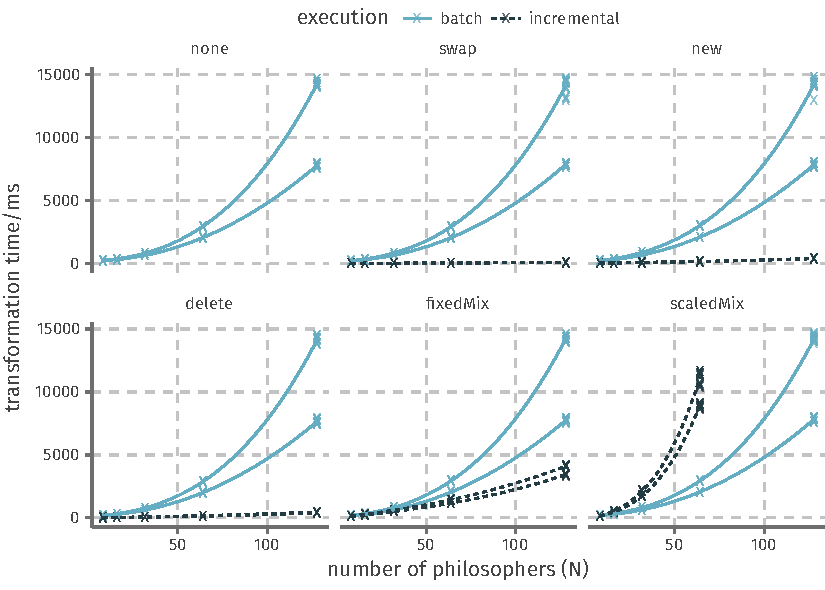
\includegraphics{figures/plot_execution}
  \caption{Execution times of transformations.}
  \label{fig:apply:plot-execution}
\end{figure}

The execution time of the transformations on the various model sizes and change operations is shown in the scatter plot in \cref{fig:apply:plot-execution}. It is apparent that the distribution of run times is extremely bimodal, especially for larger source models.

Therefore instead of fitting a single curve for each scenario, data points were split into two clusters for each scenario and model size. First the threshold \(\textit{thresh} = \frac{\textit{max} - \textit{min}}{2}\) was determined, where \textit{max} and \textit{min} were the smallest and largest execution times, respectively. Due to the heavy bimodality, no data points were adjacent to this threshold. The upper and lower clusters were then formed by data points above and below \textit{thresh}. The upper and lower curves of degree up \(3\), which are shown in \cref{fig:apply:plot-execution}, were fit to data points from the upper and lower clusters of each scenario. It is apparent that execution times of the batch scenarios in both the upper are lower clusters scale superlinearly, and the same phenomemon also occurs with incremental view synchronization of mixes of change operations. There was no correlation between the iteration numbers and the clusters, i.e.~the bimodality was not found to be a warm-up transient artifact.

\begin{table}
  \caption{Minimum and maximum execution times of transformations/ms.}
  \label{tbl:apply:minmax}
  \centering
  \begin{tabular}{@{}r*{6}{r@{\,}c@{\,}r}@{}}
    \toprule
    & & & & \multicolumn{15}{c@{}}{Incremental} \\
    \cmidrule{5-19}
    \(N\) & \multicolumn{3}{c}{Batch}  & \multicolumn{3}{c}{Swap}  & \multicolumn{3}{c}{New}  & \multicolumn{3}{c}{Delete}  & \multicolumn{3}{c}{FixedMix} & \multicolumn{3}{c@{}}{ScaledMix} \\
    \midrule
    \(8\)&\(209\)&--&\(294\)&\(6\)&\(\updownarrow\)&\(9\)&\(15\)&\(\updownarrow\)&\(26\)&\(17\)&--&\(33\)&\(126\)&\(\updownarrow\)&\(166\)&\(124\)&\(\updownarrow\)&\(163\)\\
    \(16\)&\(281\)&\(\updownarrow\)&\(344\)&\(8\)&\(\updownarrow\)&\(15\)&\(23\)&\(\updownarrow\)&\(41\)&\(27\)&\(\updownarrow\)&\(45\)&\(224\)&\(\updownarrow\)&\(291\)&\(456\)&\(\updownarrow\)&\(575\)\\
    \(32\)&\(631\)&\(\updownarrow\)&\(852\)&\(13\)&\(\updownarrow\)&\(18\)&\(46\)&\(\updownarrow\)&\(91\)&\(51\)&\(\updownarrow\)&\(86\)&\(505\)&\(\updownarrow\)&\(631\)&\(1714\)&\(\updownarrow\)&\(2221\)\\
    \(64\)&\(2006\)&\(\updownarrow\)&\(2975\)&\(26\)&\(\updownarrow\)&\(34\)&\(119\)&--&\(164\)&\(129\)&\(\updownarrow\)&\(181\)&\(1148\)&\(\updownarrow\)&\(1473\)&\(8644\)&\(\updownarrow\)&\(11\thinspace681\)\\
    \(128\)&\(7568\)&\(\updownarrow\)&\(14\thinspace659\)&\(52\)&\(\updownarrow\)&\(68\)&\(357\)&\(\updownarrow\)&\(427\)&\(383\)&\(\updownarrow\)&\(478\)&\(3342\)&\(\updownarrow\)&\(4211\) & \multicolumn{3}{c@{}}{Timed out}\\
    \bottomrule
  \end{tabular}
\end{table}

The minimum and maximum execution times of each scenario and model size, which are representative of the execution times in two clusters, are shown in \cref{tbl:apply:minmax}. Because the considered model changes did not affect the run times of batch transformations, we only report the run time of the batch transformation of the initial model. The symbol \(\updownarrow\) indicates significant (\(p < 0.05\)) bimodality of the execution time distributions according to Hartigan's dip test~\citep{Maechler16diptest}, while~--~denotes unimodal distributions.

In order to study the source of bimodality in the execution times, a further experiment was conducted. The batch transformations, which had the most striking bimodality, was executed with further instrumentation on the source model containing \(N = 128\) philosophers. Four stages of the transformation were distinguished:
\begin{enumerate*}
\item The \emph{view query} phase prepares the model queries that are the preconditions of the view transformation. In \textabbr{VIATRA} Query, this corresponds to query optimization, as well as the traversal of the source model to populate the various base relations and caches for incremental query evaluation.
\item The \emph{view transformation} phase fires the transformation rules on the \textabbr{VIATRA} Event-driven Virtual Machine (\textabbr{EVM}) to construct the abstract \textabbr{RGSPN} model with references.
\item The \emph{concretizer query} phase traverses the abstract net to prepare the precondition queries of the concretizer transformation.
\item The \emph{concretizer transformation} phase is ran on the \textabbr{EVM} to resolve references and inline expression in the abstract net to construct the concrete \textabbr{RGSPN} target model.
\end{enumerate*}
In ordinary transformation execution, the query phases are ran simultaneously to avoid spurious model traversal. Moreover, the transformation phases share an \textabbr{EVM} execution schema that provides sequential execution by prioritized firing of transformation rules. However, in our experiment, we separated the phases to observe their run times individually.

\begin{figure}
  \centering
  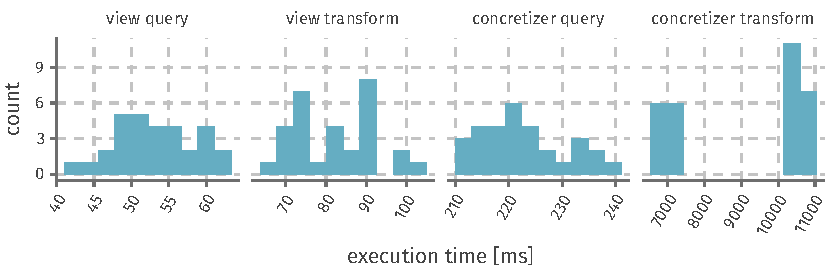
\includegraphics{figures/plot_histogram}
  \caption{Execution times of batch transformation phases with \(N = 128\) philosophers.}
  \label{fig:apply:histogram}
\end{figure}

The histogram of the transformation phases with 30~iterations is shown in \cref{fig:apply:histogram}. The concretizer transformation phase, which is running an order of magnitude slower than other phases, is revealed as the source of the heavy bimodality.

\begin{table}
  \caption{Execution times of \textabbr{PNML} serializations.}%
  \label{tbl:apply:serialization}%
  \begin{minipage}{0.5\textwidth}%
    \centering
    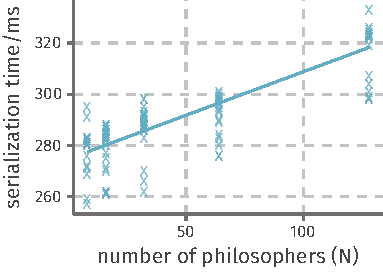
\includegraphics{figures/plot_serialization}%
  \end{minipage}%
  \begin{minipage}{0.5\textwidth}%
    \centering
    \begin{tabular}{@{}rr@{\,}c@{\,}lS[table-number-alignment=center,table-format=6.0]@{}}
      \toprule
      \(N\) & \multicolumn{3}{c}{Time/ms} & \multicolumn{1}{c@{}}{\textabbr{PNML} size/bytes} \\
      \midrule
      \(8\) & \(257\) & -- & \(295\) & 50700 \\
      \(16\) & \(261\) & \(\updownarrow\) & \(288\) & 100441 \\
      \(32\) & \(262\) & -- & \(298\) & 200572 \\
      \(64\) & \(276\) & -- & \(301\) & 400736 \\
      \(128\) & \(298\) & -- & \(333\) & 802454 \\
      \bottomrule
    \end{tabular}%
  \end{minipage}%
\end{table}

Lastly, the time taken by serialization of the target models in \textabbr{ISO}/\textabbr{IEC} \textabbr{PNML} format to an in-memory output stream is show in \cref{tbl:apply:serialization} and the accompanying figure. Both the serialization time and the size of the resulting \textabbr{PNML} descriptions scale linearly with the model size. Significant bimodality was detected by the dip test on in the case of \(N = 16\) with \(p = 0.004\). However, it is possible the latter observation is only due to pure randomness.

\subsection{Observations}

The research questions \textbf{\textabbr{RQ1}--3} may be answered based on the presented measurement results as follows:

\paragraph{\textabbr{RQ1}} Batch transformations scaled superlinearly in the size of the input model. Transformation of the largest studied source model, which had 129 elements, took up to 15\thinspace s to produce a 8452-element output model along with traceability information which affords incremental synchronization of the target \textabbr{RGSPN} according to future source model changes.

The run time exhibited significant bimodality, apparent to both visual examination an Hartigan's dip test of bimodality. In the most extreme case of \(N = 128\) philosophers, iterations in the upper cluster of run times took nearly twice as long a those in the lower cluster, while for smaller input models, the difference was up to 50\%.

\paragraph{\textabbr{RQ2}} Incremental synchronization of the \textbf{swap} change operation was found to take linear time as the function of the source model time. Therefore the synchronization time depends on not only the changes to be synchronized but also on the size of the input model. Synchronization time for \textbf{create} and \textbf{delete} changes was found to be superlinear similarly to the batch transformation. This indicates the creation and removal of objects has larger overhead than the modification of references in the source model and the \textabbr{RGSPN}.

Synchronization time was below that of batch transformation in the \textbf{fixed\-Mix} compound change operation. However, for the change operation \textbf{scaled\-Mix} of model-dependent size, batch transformation was found to be faster that incremental synchronization in all cases except \(N = 8\). Therefore we can conclude that if change operations affect large portions of the input model batch transformation may be more economical than incremental synchronization; although for smaller input changes, synchronization won by a margin of at least 14\%, the smallest difference being achieved on the \textbf{fixed\-Mix} change with \(N = 16\).

\paragraph{\textabbr{RQ3}} The \textabbr{PNML} serialization routine, which traverses the concrete \textabbr{RGSPN} model to produce its \textabbr{PNML} equivalent, scaled linearly in the size of the input model. However, the cause of this phenomemon is probably that the size of concrete \textabbr{GSPN} itself is only a constant multiple of the input model size. The size of the generated \textabbr{PNML} was also a multiple of the input model size. In all measured cases \textabbr{PNML} serialization took no more than \(\nicefrac{1}{3}\) of a second, much less than the time taken by analysis tools to analyze stochastic Petri net models similar to the ones considered. Therefore \textabbr{PNML} serialization is not a significant overhead compared to stochastic analysis. It is also generally smaller than the time taken by batch transformation.

\newpara Bimodality of transformation run time distributions was found to be caused by the execution of the \textabbr{RGSPN} concretizer transformation on the \textabbr{VIATRA} Event-driven Virtual Machine. We hypothesize that the large differences is execution time are caused by the nondeterministic scheduling in \textabbr{EVM}.

While conflicting transformation rules of differing priorities are fired in the order of their priorities, the ordering between rules of the same priority are not defined. The firing of a low-priority rule may activate a higher priority one. In the implementation of our concretizer transformation, the work performed by some high-priority rules may be occasionally undone by a low-priority rule when \textabbr{RGSPN} references are resolved and expressions are inlined due to the dependency tracking required for expression inlining. Thus if low-priority rules are fired in an unsuitable order, some work must be redone by high-priority rules after the correct dependencies are taken into account. Although taking dependencies between \textabbr{RGSPN} symbols and expressions at the level of \textabbr{EVM} conflict resolution may alleviate this issue, performing such tracking efficiently remains in the scope of future work.

Due to the hashing employed by the conflict resolver, the firing order of equal priority rules is determined at runtime by \texttt{hashCode} of the rule activation objects, which is not overridden from its default implementation. In the Java runtime environment, the default \texttt{hashCode} is connected with the allocation of objects and forcing it to be deterministic for the sake of consistent measurements is difficult. Hence the apparently random switching between fast and slow execution of the concretizer transformation.

\subsection{Threats to validity}

An internal threat to validity was the possibility of an incorrect implementation of the transformation engine or the incorrect description of the transformation from the dining philosophers domain model to Petri nets. To ensure correctness the transformation outputs were manually inspected for the small source models for consistency with the source models and the transformation description.

Moreover, interferences may have occurred in the measurement environment. To reduce interferences, the measurements were ran on a physical machine on which no other task was executed at the time. Each scenario and input model was measured 30 times after 10 warm-up iterations to reduce random noise and the interferences caused by ongoing just-in-time compilation. Garbage collection within the runtime environment was also controlled manually to ensure that subsequent iterations did not interfere.

Despite these attempts, run time distributions were found to be bimodal having two clusters with small variance instead of a single cluster with small variance. We conducted further measurements to break down the transformation into phases and hypothesize that this phenomenon is intrinsic to the current implementation of the transformation instead of being caused by interferences.

As we conducted our experiments on in single domain with a single transformation description, several external threats to validity impede generalization. Firstly, further studies are needed to observe the behavior of the transformation on different domain models and transformation descriptions. Secondly, as the size of the target \textabbr{RGSPN} models was a constant multiple of the size of the source models, behaviors depending on the sizes of either of these models could not be distinguished from each other.
